\graphicspath{{Images/intro/}}
\chapter{introduction}
\label{chap:intro}

%\def{pdf}
%\ifpdf
    %\graphicspath{{Chapter1/Figs/Raster/}{Chapter1/Figs/PDF/}{Chapter1/Figs/}}
%\else
    %\graphicspath{{Chapter1/Figs/Vector/}{Chapter1/Figs/}}
%\fi
Traditionally, robots are made of rigid materials such as steel. Rigidity enables the robots to perform repeated tasks with high speed and precision. Rigid robots are usually designed for a specific task and they are therefore, not suitable if there is a change in the working conditions. Biological organisms on the other hand, can perform a much wider range of tasks, although with lower precision and speed. Therefore, scientists have been inclined towards using soft materials in robots in order to make them more similar to soft living organisms in terms of adaptability.~\subfigref{fig:venn}{a} is an example of a soft robot that can perform grasping of delicate objects without damaging them regardless of their shape or surface roughness~\cite{Li2019}.

Untethered robots are a class of robots that can function independently without any connection to external power supplies or other equipment. Therefore, untethered robots can be used as autonomous mobile robots. Boston Dynamics' Atlas\footnote{https://www.bostondynamics.com/atlas\label{fn:boston}} can be considered as an example of untethered robots as can be seen in~\subfigref{fig:venn}{b}. 

Miniature robots have application in exploring tight spaces such as inside human body. Since miniature robots use less material, and their fabrication methods are less costly, they can be manufactured in large scale and be used in swarm robotics. The mentioned three categories of robots can be combined to make robots that have advantages of each category.~\subfigref{fig:venn}{c,d,e} are examples of such robots. As an instance~\subfigref{fig:venn}{c} shows a low cost miniature insect robot that can be used in large numbers to pollinate plants~\cite{Jafferis2019}. 

Finally, there are miniature, untethered soft robots that take advantage of all categories and are the focus of this dissertation as shown in~\subfigref{fig:venn}{f}\textcolor{red}{khodambashi~\cite{}}.
 
%In this chapter, the reasons that justify the use of soft robots are discussed. Then the limitations of current soft robot technologies are presented, followed by an overview of the problems that are addressed by this thesis. 
\begin{figure*}[!ht]
      \centering
      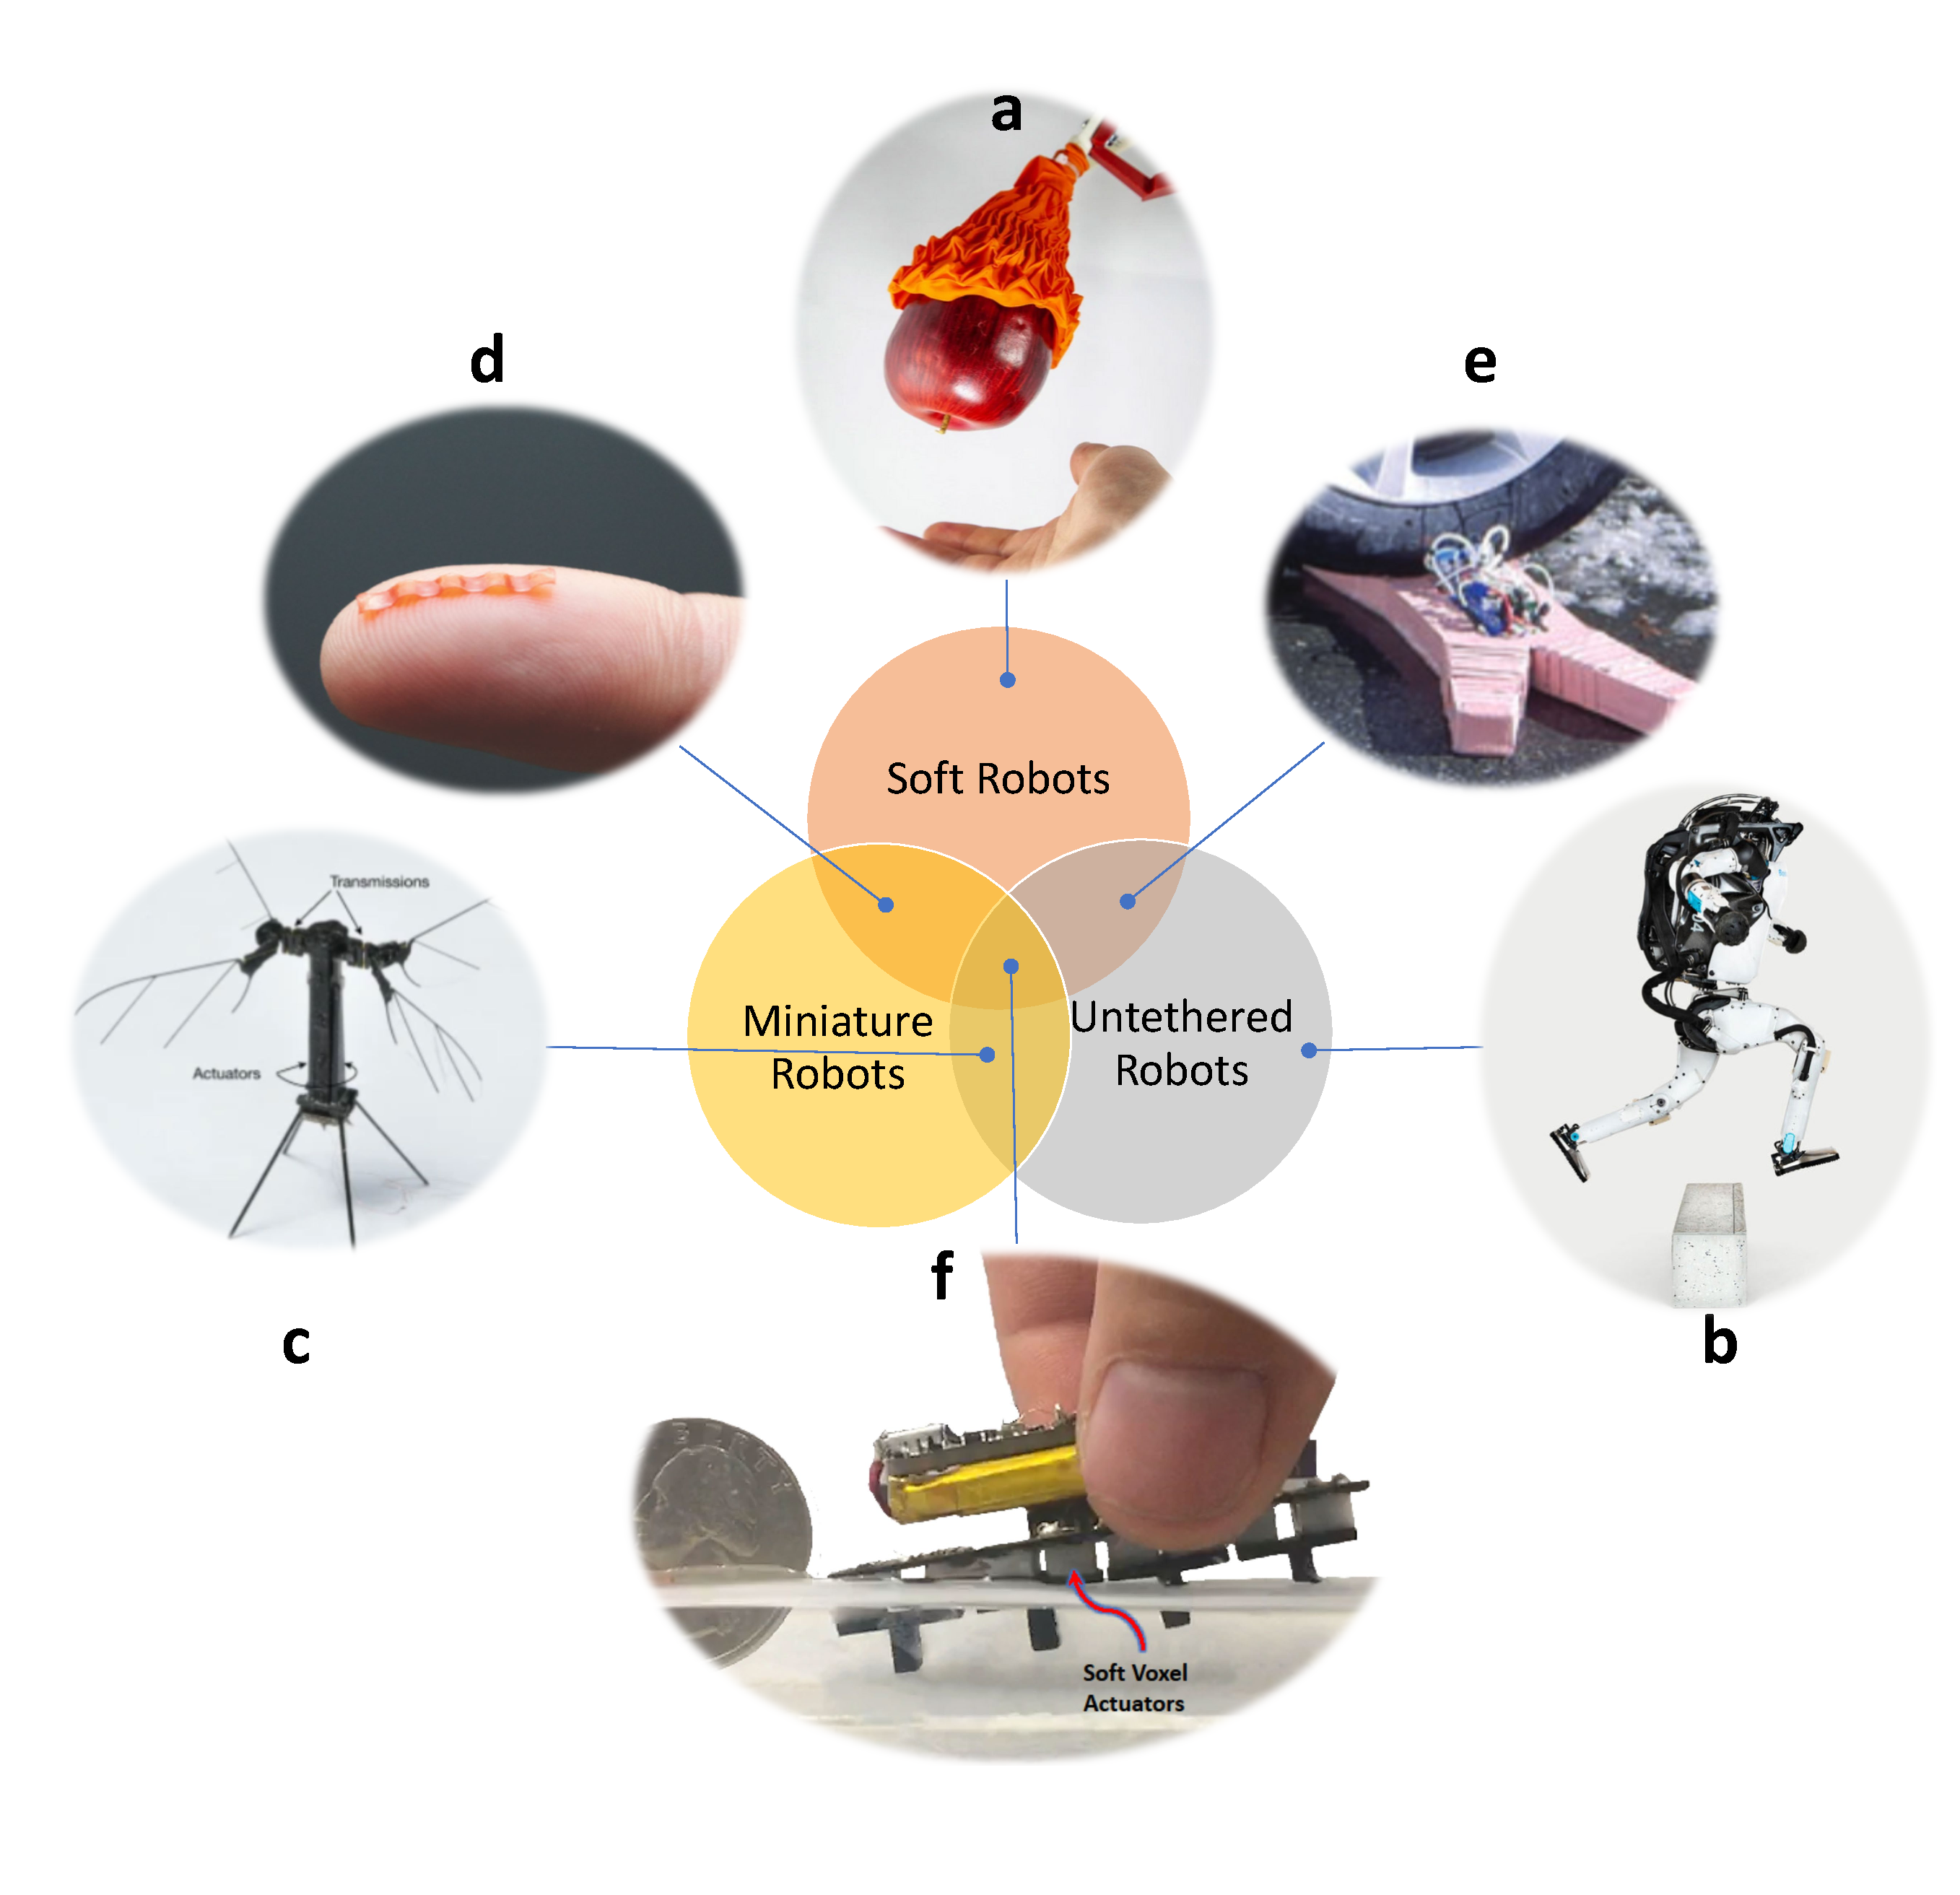
\includegraphics[width=\textwidth]{venn.pdf}
      \caption{Classification of robots. a) soft robot~\cite{Li2019}. b) Untethered robot~\footref{fn:boston} c) Miniature untethered robot~\cite{Jafferis2019} d) Miniature soft robot~\cite{Tingting2012} e) Untethered soft robot~\cite{Tolley2014d} f) Miniature untethered soft robot\textcolor{red}{khodambashi~\cite{}}}
      \label{fig:venn}
\end{figure*}

\section{Soft Robotics as an Emerging Field}
\label{sec:emerging}
Majority of biological organisms contain soft tissue. The soft tissue brings some advantages to these organisms. Octopus is the most widely used source of inspiration for soft robotic research. Octopuses can deform their body and pass through small openings. Therefore, shape morphing is one of the key advantages of soft organisms. Octopuses can also soften their arm as they wrap it around a bottle cap and stiffen their arms for a tight grip as they turn the cap to open it as shown in Fig. Variable stiffness is therefore, another aspect of soft organisms. Human hand is another example which can demonstrate some of the advantages of compliant materials. Human hand can grasp objects with a wide range of shapes and surface roughness without slipping because the soft tissue passively conforms to different shapes (Fig). Human hand can also absorb energy from an impact such as catching a baseball, preventing any damages to the hand. Impact tolerance is another key advantages of soft bodied organisms. The ability to absorb the impact energy also protects the surrounding objects and humans in case of a collision. This brings up safety as another important feature of compliance present in soft bodied animals. The advantages of soft animals are summarized in Table. Inspired by biology, soft robot developers try to utilize the advantages inherent in soft, compliant matter to achieve safer interactions around humans or more robust locomotion and manipulation in unstructured environments~\cite{martinez2013,laschi2012,Tolley2014d,AdamBilodeau2015}.

\section{State of the Art in Soft Robotics}
Traditionally, robots were made to be stationary. They were unaware of their surroundings and operated based on a prescribed set of instructions. Recent advances in sensor technologies have paved the road to mobile autonomous robots which here, are categorized as untethered robots. Therefore, in addition to soft actuators, sensors and computers are also an integral part of any untethered robotic system. For a soft robot, ideally all these components should be soft. Here, the state of the art technology in each category is reviewed with a special attention paid to the soft actuators which is the focus of this dissertation. 
%Soft robots are categorized based on many different features. Here, we focus on miniature and untethered robot categorization to stay focused on the topic of this thesis. Since manufacturing is part of the contribution of this thesis, a brief survey of the manufacturing techniques is also presented.
%\subsection{Components of a Soft Robot}
\subsection{Soft Sensors}
The research on soft sensors focuses mainly on the stretchable sensors for wearable health monitoring~\cite{Liu2017c,Amjadi2016a}. Since these sensors have desirable characteristics, researchers have started to use these sensors in soft robots. Sensors based on liquid metals have particularly been successfully implemented to measure the strain in soft silicon-based devices~\cite{Hammond2014,Chossat2013, Wang2019c,Ren2020}. Other sensor technologies are piezoresistive~\cite{Georgopoulou2020,Turgut2018,Melnykowycz2016}, capacitive~\cite{Hohimer2020,Cao2020,White2017,Frutiger2015}, and conductive polymers~\cite{Chen2021,Kanoun2021,Harito2020}. Majority of these sensors work based on the change in resistance of the material when they undergo strain. 
\subsection{Soft Computers}
Traditionally,  majority of the computations happen on microcontrollers made of hard materials. This is unavoidable and is one of the major limiting factors in the development of entirely soft robots. Soft computers are in their incipient stage. They are based on pneumatic circuits and can perform simple logic functions~\cite{Preston2019,Garrad2019}. Another research direction is using the living cells as computers~\cite{Daniel2013}. This area also needs significant development before it can be successfully implemented in the structure of soft robots. 
\subsection{Soft Actuators}
Actuation is the core of a robot and as such, there is a larger amount of research on soft actuators as compared to soft sensors and computers. Soft pneumatic actuators (SPAs) \cite{Gorissen2017, Branyan2018} are the most widely used category of actuators in soft robotics. They are based on a chamber made of soft materials which is pressurized using fluids. The chamber deforms as a result and produce motions such as bending, elongation or twisting. SPAs have high power to weight ratio and have relatively fast response.  Another class of actuators use active materials that undergo a strain based on a stimulus. This class includes shape memory alloys (SMAs)\cite{Cianchetti2014}, dielectric elastomer actuators (DEAs)~\cite{Carpi2008,Gu2017}, liquid crystal elastomers (LCEs)~\cite{Kularatne2017,Yu2015a}, and stimuli-responsive hydrogels~\cite{Calvert2009,Liu2020,Ionov2014,Banerjee2018}. 
 
%\subsection{Untethere d Soft Robots}
%For functioning as mobile robots, the essential accessories such as pumps or power supplies need to be embedded in the robot itself. These robots fall under the category of untethered soft robots [].  
%\subsection{Miniature Soft Robots}
%Miniature robots have dimensions under...and have a low load carrying capacity. These robots have applications where small loads need to be applied, in working with delicate objects, or in tight environments such as inside human body. 
%\subsection{Miniature Untethered Soft Robots}

%\subsection{Soft Robot Manufacturing Techniques}
%\subsubsection{Molding}
%\subsubsection{3D Printing}
\section{Challenges Ahead}.
Initially, the focus of soft robotics was to find manufacturing methods for SPAs and assemble them into functioning prototypes. These robots were made for tasks such as grasping or used as stationary continuum manipulators. In these applications, the size and weight of the accessories is less important because the accessories are located near the robot and does not have to be carried by the robot. In case of mobile robots however, it is necessary to include all the accessories within the robot and therefore, careful design is required to meet the weight limitations. This challenge becomes more serious in case of miniature robots. SPAs use passive materials such as silicone and rely on rigid components such as motors and pumps that are difficult to downscale and therefore, manufacturing small-scale soft actuators which have applications as envisioned by \cite{hines2017} has remained a bottleneck in the development of miniaturized soft robots \cite{majidi2019}. This category of soft robots are least explored due to complicated materials and fabricating processes. Small-scale actuators can be produced using responsive materials such as DEAs, LCEs and hydrogels. These actuators lack sensing and computation which are essential subsystems of a true robot and are usually used in a human-in-the-loop scenario where sensing and computation are performed by a human operator. This helps in down scaling the robots to the micrometer range. These actuators can perform limited robotic functions and have highly specific applications such as to perform a colon tissue biopsy. However, these robots can not function as autonomous robots because they lack sensing and computation and rely on external devices for their operation. For instance,~\cite{Palagi2016} needs a light projecting device to generate the light patterns required for creating deformations and movement in a light-responsive actuator. Another example is a magnetic-responsive actuator~\cite{Kim2018} which rely on a magnetic field generator for its operation. All these equipment are bulky and require careful setup and therefore, these types of actuators are not suitable for use in autonomous mobile robots. Technologies are still needed to create small-scale autonomous soft robots that function similar to biological organisms such as annelids, mollusks, and octopuses. Considering the highly sophisticated structure of living organisms, simultaneous progress in multiple disciplines such as materials science, design, manufacturing and control is required in order to achieve soft robots that are closer to their biological counterparts.

Hydrogels are close to soft tissue in terms of material properties and the muscle like contractions in response to external stimuli~\cite{Liu2020}. Also, they can be made to be ion conductive and biocompatible. These features can add up to the benefits of soft robots namely safety and adaptability~\cite{Lee2020}. However, the uniform responsive volume change of bulk hydrogels makes it less interesting in robotic applications, which instead demands complex spatiotemporal reconfigurability~\cite{Erol2019} - as the dexterous octopus arm presents. The challenge is to create 1) on-demand, 2) time-varying and 3) local deformations in a hydrogel structure. From a structural design perspective, the majority of reported heterogeneous hydrogel structures demonstrate fixed deformation patterns, such as static shape shifting of sheets without any interaction with the environment~\cite{SydneyGladman2016, Ma2019, Jeon2017} or bending of beams to perform simple gripping functions ~\cite{Wang2017, Ma2018, Duan2017} Only a few methods demonstrate on-demand deformations and are able to interact with objects~\cite{Mourran2017, Palagi2016, Kim2018} but involve bulky equipment (light and magnetic field generators), making them impractical for mobile soft robots or embedded applications.
From a materials perspective, there is a need for a powerful but simple synthesis method to broadly tune the material response behavior (volume changing ratio, speed, and stiffness), to meet the requirement of creating a complex robotic structure with spatiotemporal reconfigurability.

\section{Contributions of this Dissertation}
This dissertation demonstrates progress in different areas of material science and manufacturing  that together, will contribute to the field of soft robotics. A set of design decisions are made based on closed collaboration of teams of material scientists and roboticists which helps the informed progress of one field by considering the requirements of the other. A bioinspired approach is used to help with some of the design decisions. Biological organisms use electrical signals from the nervous system in conjunction with responsive muscle tissue to perform soft actuation. This combination helps them to be self-contained and also, it is viable across scales from giant octopuses to millimeter-sized worms. Therefore, the first feature that is considered for the design of soft robots is to use a material that is responsive to electrical stimulus. The living organisms also are made of cells which are simpler building blocks assembled to form a more complex organ. The second requirement imposed is therefore, to use a bottom-up strategy to fabricate complex robots using simple building blocks that are easy to manufacture. The contribution of this dissertation as shown in Figure~\ref{fig:summary} can be summarized as follows:

\begin{itemize}
	\item A novel, temperature-responsive hydrogel material with fast response. This material functions as artificial muscle tissue. 
	\item A Facile and tunable synthesis method. This makes the synthesis method simple and accessible by the soft robotics community which have less access to material processing facilities.
	\item A voxel-based assembly approach. This helps to use simple building blocks called soft voxel actuators (SVAs) to assemble more complex soft robots. SVAs are easy to manufacture and solve some of the challenges associated with embedding electronics in soft robots.
	\item Electrical Joule heating of SVAs. This enables the use of small footprint microcontrollers and paves the road to embedded and mobile robot applications.
	\item Realization a hyper-redundant hydrogel-based electrically addressable miniature soft robots capable of performing tasks that require high number of DOF. High dexterity and the ability to function in unstructured environments are functionalities, which separates our devices from previously demonstrated structures.
	\item Realization of a miniature untethered soft robots. This robot weighs only 20g including battery and power supply and does not rely on external equipment or human intervention for its operation.
\end{itemize}
\begin{figure*}[!ht]
      \centering
      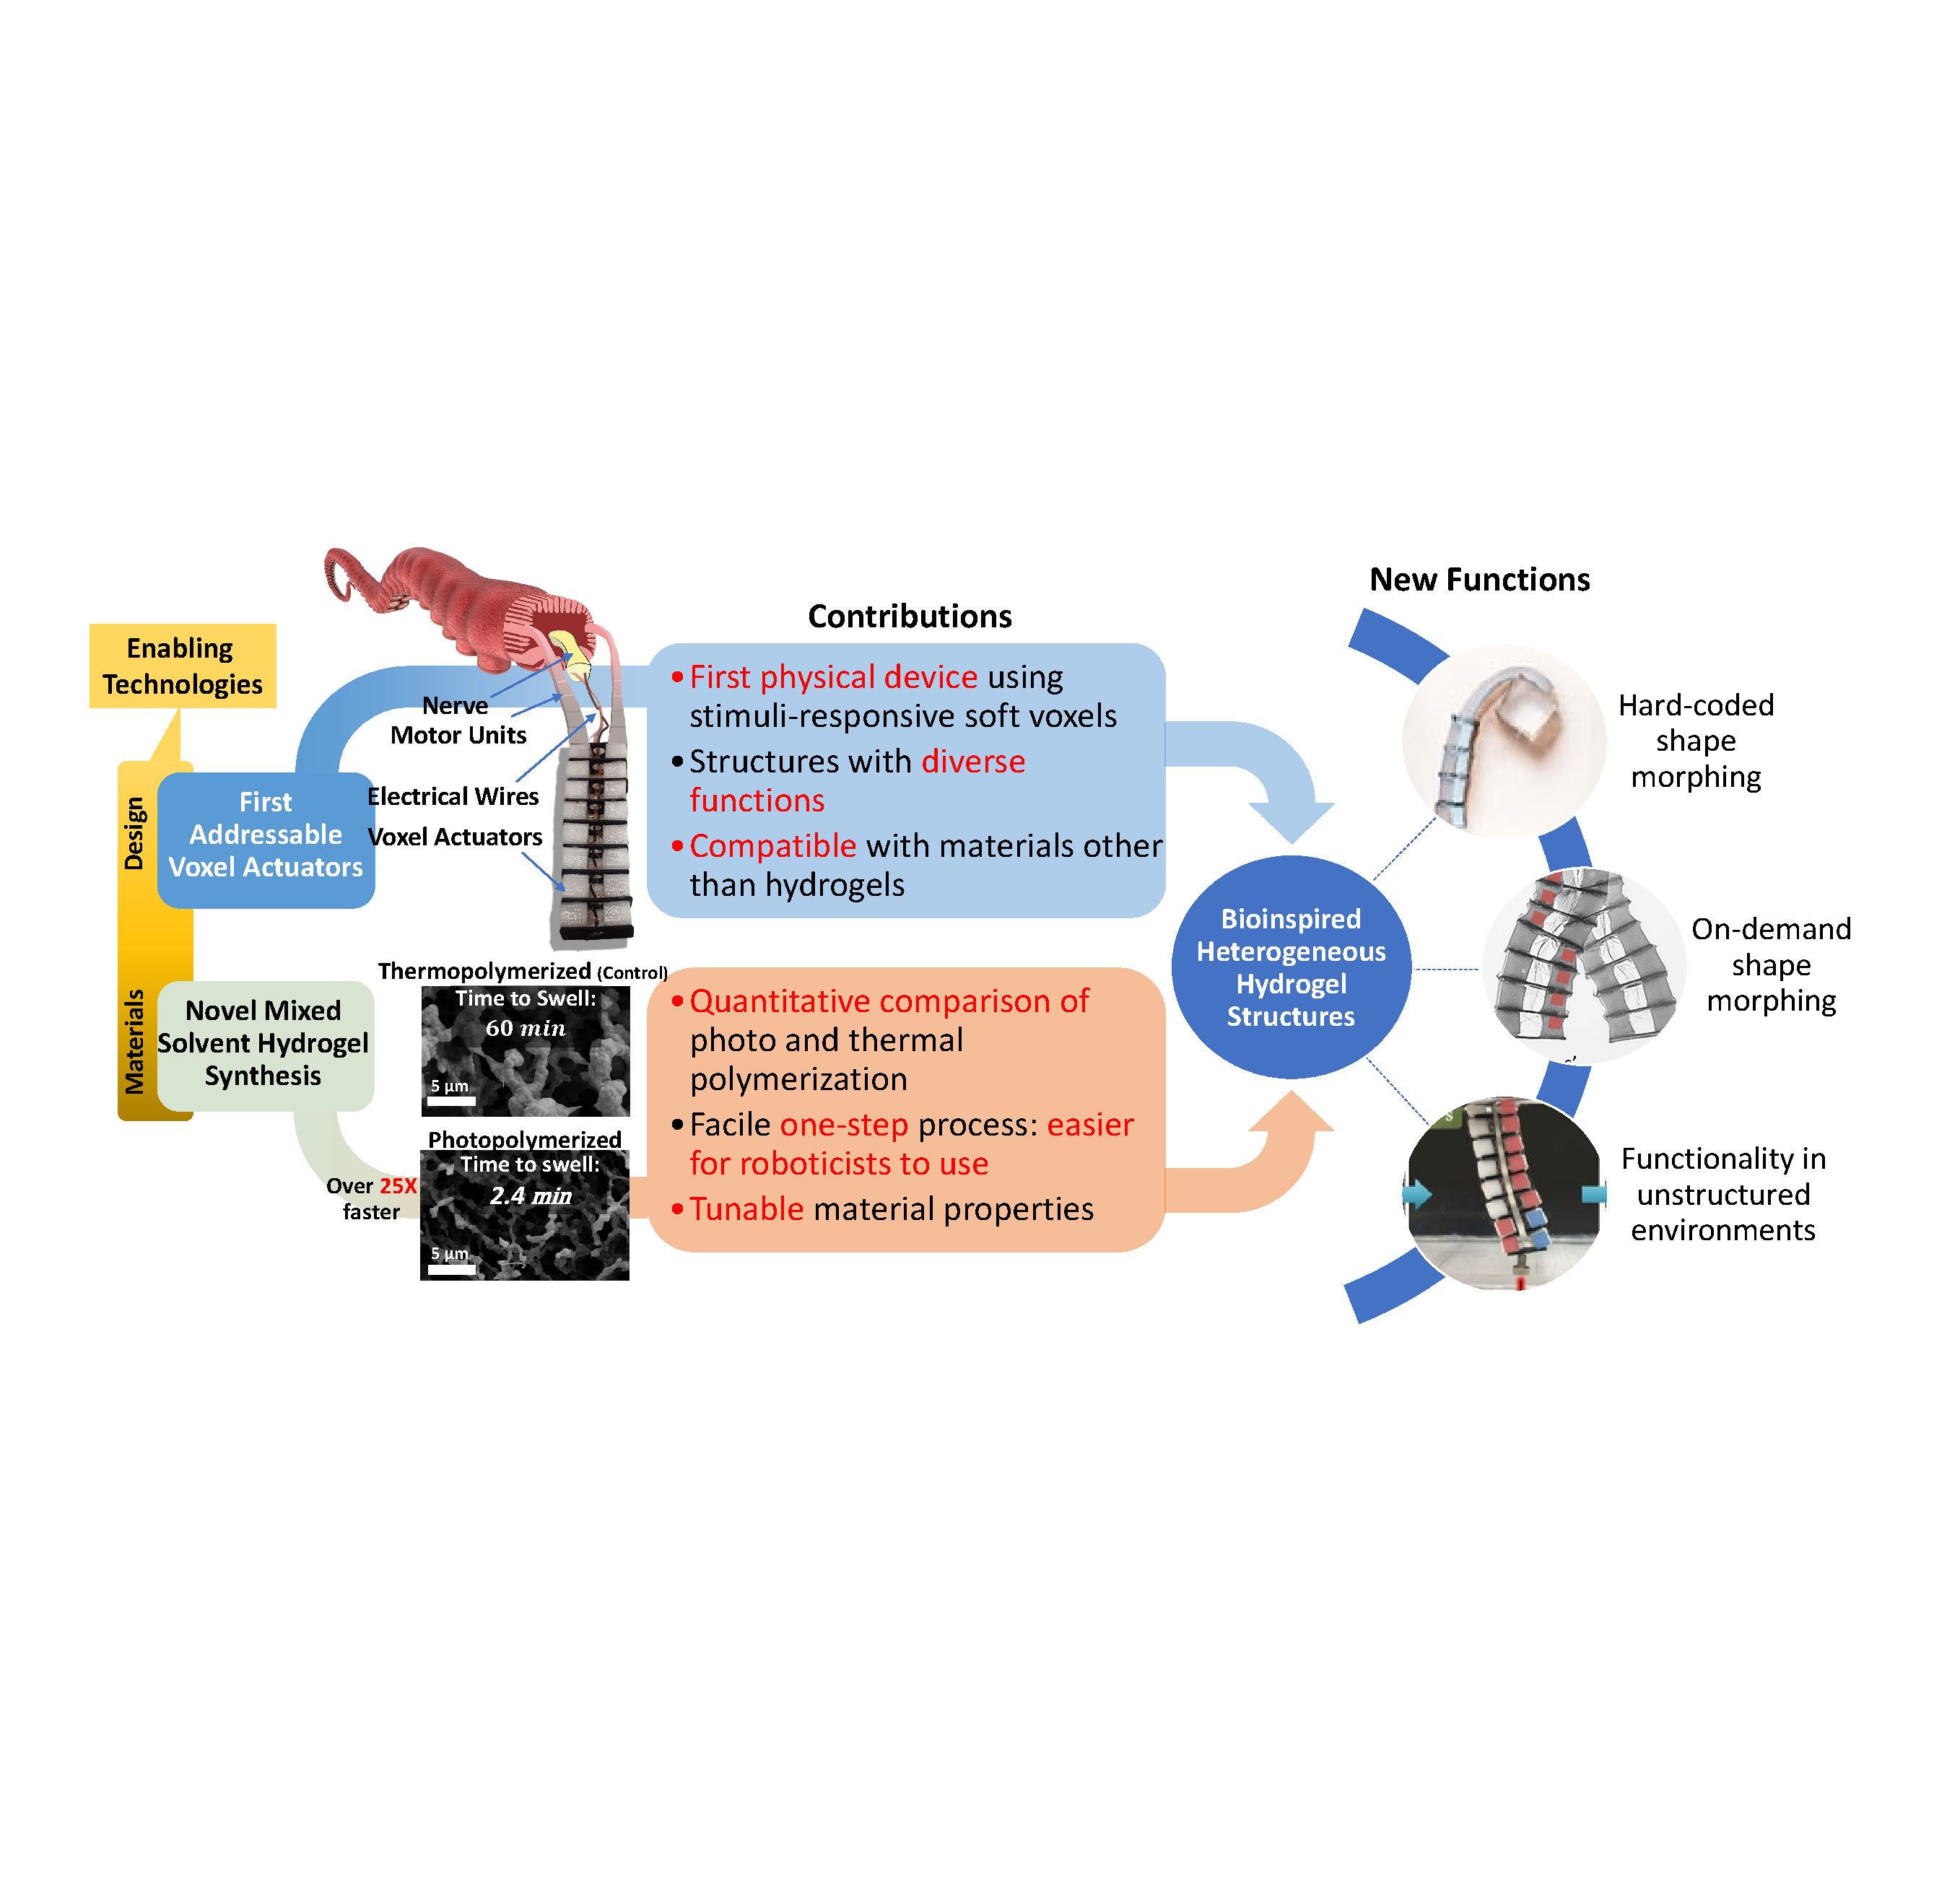
\includegraphics[width=\textwidth]{summary.pdf}
      \caption{Classification of robots. a) soft robot~\cite{Li2019}. b) Untethered robot~\footref{fn:boston} c) Miniature untethered robot~\cite{Jafferis2019} d) Miniature soft robot~\cite{Tingting2012} e) Untethered soft robot~\cite{Tolley2014d} f) Miniature untethered soft robot\textcolor{red}{khodambashi~\cite{}}}
      \label{fig:summary}
\end{figure*}
%\subsection{Broader Impact}
%\subsubsection{Scientific}
%Current soft actuators rely on additional hardware such as pumps, high voltage supplies, light generation sources and magnetic field generators for their operation. These components resist miniaturization and embedding them into small-scale soft robots would be challenging. This limits their mobile applications especially in hyper-redundant robots where a high number of actuators are needed. On the other hand, our developed SVAs weigh only 100 mg and require small footprint microcontrollers for their operation which can be embedded in the robotic system. 
%\subsubsection{Social}
%Soft robots are intrinsically safe around humans. This can help bring robots to daily life applications such as household robots and assistant robots for elderly people. Also, our soft robots can operate underwater due to hydrogel compatibility with moist environments. A swarm of soft robots can be used for underwater exploration and data collection and help monitor the climate change through recording the water current temperatures over long period of time.

\subsection{Dissertation Outline}
The following chapters discuss the innovations in materials science and manufacturing methods that lead to the development of miniature untethered soft robots.\\ 
\textbf{Chapter~\ref{chap:SVAs}: Soft Voxel Actuators: Hydrogel Building Blocks for Bottom-up Assembly of Soft Robots}\\
This chapter discusses the recipe for preparing temperature-responisve hydrogels. Improvements have been made in the synthesis technique such that it is more accessible to robotic researchers who have less access to material processing facilities. In addition, this recipe results in hydrogels with fast response, solving a challenge that has limited the use of hydrogels in soft robotics. Next, building blocks called soft voxel actuators (SVAs) are introduced that facilitate the manufacturing of soft robots through a bottom up assembly approach. Both the hydrogel and SVAs are characterized in-depth in terms of material properties and actuation properties.
  
\textbf{Chapter~\ref{chap:heterogeneous}: Heterogeneous hydrogel structures as Miniature Hyper-redundant Soft Manipulators}\\
This chapter is case study I of the application of SVAs and is focused around miniaturizing soft robots without loosing their functionality as a result of reducing the number of degrees of freedom. Hyper-redundant miniature soft robotic manipulators are developed. It is shown that the use of SVAs facilitates the development of such robots. These robots are able to work in unstructured environments where the working conditions might change. This manipulator has 16 actuators in a ... footprint which is the highest reported number of degrees of freedom in a miniature robot of this dimension.

\textbf{Chapter~\ref{chap:untetheredWalker}: Miniature Untethered Underwater Walking Robot}\\
This chapter is case study II of the application of SVAs and is focused around the development of untethered miniature robots. It is demonstrated that the use of SVAs can significantly reduce the weight and size of the robots. These robots are fully untethered which means all the electronics and the power source is included in the robot. 

\textbf{Appendix~\ref{chap:control}: Tracking Control of a Miniature 2-DOF Manipulator with Hydrogel Actuators}
The electrical stimulation of SVAs inspired by biology has many advantages and open the doors to equip the robots with artificial intelligence. As a first step, the automatic control of the SVAs using a microcontroller is presented in this chapter. Instead of turning the SVAs on and off as explained in Chapter~\ref{chap:heterogeneous}, the deformation of SVAs are controlled using a closed-loop control system based on the feedback from vision sensors which record the desired output of the system. A 2-DOF manipulator is fabricated using two SVAs and the position of the tip of the manipulator is controlled. As the final demonstration, a starfish inspired robot is presented which can carry a payload. The closed-loop control helps the payload transport to reach a higher speed compared to an open loop control. 

